This chapter describes how we realized the formal framework developed in \cref{ch:choreography_language} into an executable prototype. To this end, we present \textsc{ARIA}\footnote{The complete source code of \textsc{ARIA} is available at: \url{https://github.com/JTuerker/ARIA}} (Automated Reasoning for Interactive Choreographies), a tool that systematically explores choreographic executions and derives the corresponding Markov chain in an automated and efficient manner.

\section{Goal of the Implementation}
The goal of the implementation is to make the formal framework established in \cref{ch:choreography_language} practically usable. While the theoretical model shows that choreographies give rise to Markov chains, applying this construction to realistic systems requires an automated exploration procedure that can systematically capture large and complex state spaces.
We address this challenge with \textsc{ARIA} by providing an automated pipeline from high-level choreographic specifications to stochastic models.

Specifically, we designed the implementation to achieve the following four objectives:

\begin{enumerate}
	\item \textbf{Automated State-Space Exploration:} We aim to explore all reachable configurations $(S,C)$ of a choreography in a systematic manner. To this end, we implemented the operational semantics using a worklist-based exploration algorithm, which allows us to construct the reachable state space automatically.
	
	\item \textbf{Direct Model Generation:} We focus on the direct construction of the state-space from the operational semantics. By generating states and transitions without relying on an intermediate high-level modeling language, we ensure a precise mapping between our formal model and the resulting stochastic process. This approach allows us to avoid the overhead of an additional compilation step and the necessity of encoding complex, unbalanced control flow into the restricted syntax of guarded command languages.
	
	\item \textbf{Semantic Fidelity:} We ensure that the implementation remains closely aligned with the formal semantics. We designed \textsc{ARIA} such that each generated transition corresponds to a valid application of the inference rules defined in \cref{sec:semantics}. This ensures that the deadlock-freedom-by-design guarantees of our model are preserved in the generated output.
	
	\item \textbf{Interoperability and Validation:} Finally, we ensure that the generated model is fully compatible with established verification tools. We achieve this by exporting the state space into the PRISM explicit format, specifically using the \texttt{.sta} (state) and \texttt{.tra} (transition) file extensions. This interoperability allows us to use \textsc{ARIA} as a specialized front-end for choreographies while leveraging the PRISM model checker for the subsequent analysis and validation.
\end{enumerate}

\section{System Architecture}
We implemented \textsc{ARIA} as a standalone Java application. Its architecture follows a staged pipeline consisting of a \textit{front-end} for choreography processing, a \textit{back-end} for state-space exploration, and a \textit{post-processing} step for serialization to model-checker formats. Java was chosen as the implementation language because it offers a practical balance between portability, type safety, and performance for a compiler-like analysis tool. The project is managed with \textsc{Maven} to support consistent dependency management and reproducible builds.

For the \textit{front-end}, we utilize \textsc{ANTLR4}~\cite{antlr4} as a parser generator to process choreography specifications. Based on the context-free grammar provided by Carbone and Veschetti~\cite{CarboneVeschetti} (see \cref{sec:grammar}), we employ \textsc{ANTLR4} to generate the lexer and parser. We then recursively traverse the resulting parse tree with a custom visitor to construct an Abstract Syntax Tree (AST). This AST serves as our internal representation of the input choreography for the subsequent state-space exploration. 

The back-end of ARIA is centered around a worklist-based state-space exploration engine. We chose an iterative approach over a recursive implementation for two reasons. First, it avoids Java’s call-stack limitations when exploring deep state spaces. Second, it decouples successor generation from the exploration order, allowing the scheduling policy to be varied independently of the semantic rules.
This design proved essential for handling state-space explosion. The iterative worklist-based design decouples successor generation from the exploration order. This flexibility allows the engine to employ a \textit{biased hybrid search strategy}, which can be tuned to balance between different traversal policies depending on the model's complexity (see \cref{sec:efficiency}).

Starting from an initial configuration $(S,C)$, the exploration engine incrementally computes successor states by applying the operational semantics defined in \cref{ch:choreography_language}. To avoid redundant exploration and ensure termination, visited configurations are stored in a centralized hash-based data structure for efficient state deduplication. This is essential for explicit-state generation, since the same global configuration may be reached through different concurrent execution paths. To further optimize performance-critical operations, we employ specialized collection classes from the \textsc{FastUtil} library. By using custom hashing strategies and avoiding the overhead of standard boxed collection types, we reduce heap usage and accelerate state lookups, especially for large state vectors where equality must be determined by content rather than object identity.

To interface with probabilistic model checkers, each discovered configuration is assigned a unique numerical identifier. Serialization into the PRISM explicit format (\texttt{.sta} and \texttt{.tra}) is performed as a separate post-processing step after exploration has concluded. This separation ensures that the available memory is primarily dedicated to state-space exploration, without additional overhead from I/O operations and string formatting during the search phase.

Finally, the implementation is maintained in a Git-based version control system in order to support traceability and reproducibility of further development.


\section{Realization of the Theoretical Model}
This section describes the realization of the theoretical model, bridging the gap between formal semantics and technical execution. To provide a coherent guide through the implementation details, we again use the \texttt{VendingMachine} protocol as a running example, this time in a recursive variant that models continuous operation (see \cref{lst:vending-machine-recursive}).

\begin{listing}[h]
	\begin{minted}{text}
		preamble
		"ctmc";
		"const int price = 2;"
		endpreamble;
		
		user -> user : "money=0";
		machine -> machine : "snack=0", "change=0";
		
		{
			Start :=
			if "money < price" @user then {
				["1.0"] "money'=money+1" @user .
				Start
			} else {
				Payout
			}
			
			Payout :=
			if "money >= price" @machine then {
				machine -> user : (
				+ ["0.9"] "snack'=1, money'=0" . Start
				+ ["0.1"] "snack'=0, change'=1, money'=0" . Start
				)
			}
		}
	\end{minted}
\caption{The recursive \texttt{VendingMachine} protocol}
\label{lst:vending-machine-recursive}
\end{listing}
Lines 13 and 14 realize the recursive continuation of the protocol: after completing the \texttt{Payout} phase, both probabilistic outcomes transition back to the \texttt{Start} protocol, allowing the process to re-enter its initial waiting state and handle further user inputs indefinitely. From a technical perspective, this recursive definition implies that the induced state-space representation contains cycles rather than terminating after a single interaction. This provides a critical test case for our compiler: the exploration engine must correctly identify previously visited state vectors and avoid re-expanding them indefinitely. Only then can the exploration terminate once the finite set of reachable states has been exhausted.

To bridge the gap between this textual specification and the automated generation of the states and transitions, the compiler first translates the input protocol into an Abstract Syntax Tree (AST). As shown in \cref{fig:ast-vending-machine}, this hierarchical representation breaks down the high-level syntax into structured components, including the preamble, role definitions, and control-flow nodes.

\begin{figure}[h]
\centering
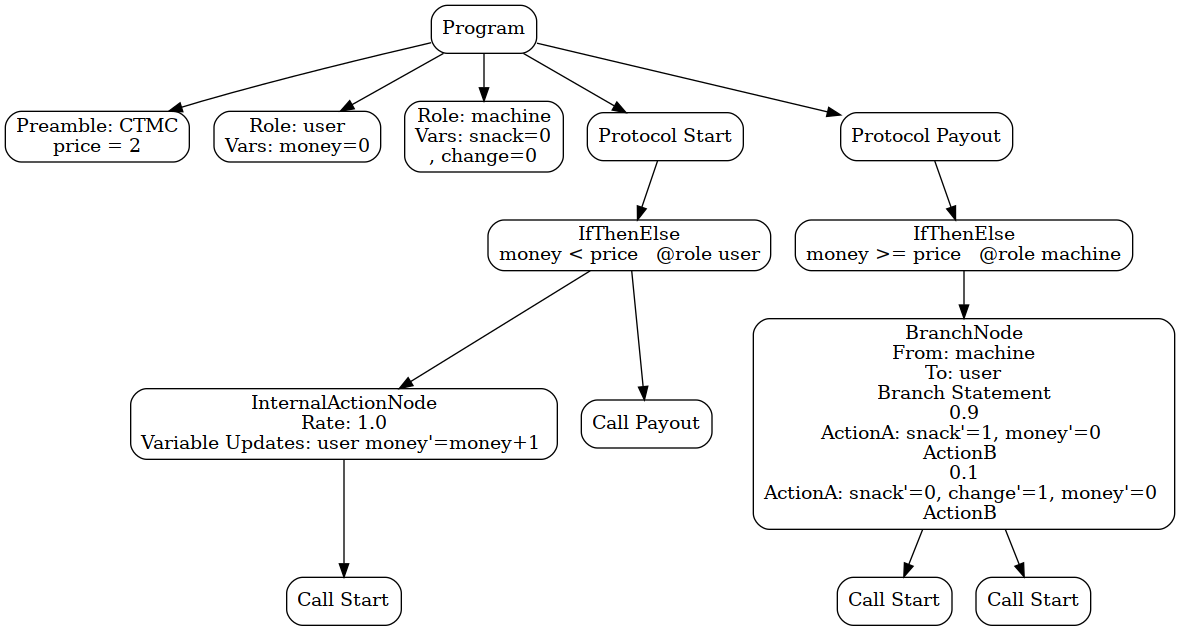
\includegraphics[width=0.9\textwidth]{figures/vendingMachine.png}	
\caption{AST representation of the Vending Machine protocol: each node within the tree is assigned a unique numeric identifier (\texttt{pcId}) during the compilation process. These IDs allow the engine to track the progress of each process by storing the current node's identifier in the program counter segment of the state vector.}
\label{fig:ast-vending-machine}	
\end{figure}
The AST representation is fundamental for the exploration engine: each node within the tree is assigned a unique numeric identifier (\texttt{pcId}) during the compilation process (see \cref{subsec:vector-representation}).
\subsection{State Vector Representation}
\label{subsec:vector-representation}
To manage the state efficiently, we represent the abstract state $S$ as a flat \texttt{Object[]} array in memory. We partition this vector into two distinct logical segments: the \textit{program counter} segment and the \textit{variable} segment. 

The Program Counter (PC) segment stores the current control location for each active process. We manage the mapping of process names to their respective vector indices using the  \texttt{process\-Name\-To\-Pc\-Index} map. During initialization, we define the boundary for the following segment by setting the \texttt{variable\-Section\-Start} offset, which corresponds to the total number of processes in the system (see \cref{lst:pc-mapping}). 
\begin{listing}[h]
\begin{tcolorbox}[
	colback=white,          % Hintergrund weiß
	colframe=gray!50,         % Rahmenfarbe schwarz (oder gray!50 für dezenter)
	arc=0mm,                % Eckige Kanten
	boxrule=0.5pt,          % Dicke der Linie
	left=0mm, right=0mm, top=1mm, bottom=1mm, % Innenabstände der Box
	boxsep=0mm
	]
\inputminted
[linenos, 
firstline=71, 
lastline=72
]{java}{code/MatrixBuilderOnTheFlyWithStateVectors.java}
	
\vspace{-0.7em} \centering \textcolor{gray!60}{$\vdots$} \vspace{0.3em}
 % Block 2: Prozess-Mapping und Segment-Grenze	
\inputminted[
linenos, 
firstline=89,        
lastline=102,         
]{java}{code/MatrixBuilderOnTheFlyWithStateVectors.java}


\vspace{-0.7em} \centering \textcolor{gray!60}{$\vdots$} \vspace{0.3em}

% Block 4: Finale Vektor-Groesse
\inputminted[frame=none, firstline=110, lastline=110]{java}{code/MatrixBuilderOnTheFlyWithStateVectors.java}
\vspace{-0.4em}
\inputminted[frame=none, firstline=111, lastline=111]{java}{code/MatrixBuilderOnTheFlyWithStateVectors.java}
\end{tcolorbox}
\caption{Initialization of the Program Counter mapping}
\label{lst:pc-mapping}
\end{listing}

A key characteristic of our implementation is the dynamic assignment of numeric IDs to AST nodes. Unlike static instruction pointers, these IDs are generated at runtime during each exploration run. Importantly, the IDs do not identify the type of a statement, but its concrete position in the program tree. Thus, even if two syntactically identical statements appear consecutively in the choreography, each receives its own \texttt{pcId}, because they correspond to different locations in the AST.

To support this encoding, we maintain a bidirectional mapping. The \texttt{nodeToPcId} map translates AST node references into numeric identifiers stored in the state vector, while the \texttt{pcIdToNode} list resolves such identifiers back to their corresponding AST nodes during interleaving. In addition, one distinguished ID is reserved for terminal or \texttt{null} states in order to represent process termination. Although the concrete numeric values of the assigned IDs may vary between different executions of the compiler, they remain stable throughout a single exploration run.

\begin{figure}[ht]
	\centering
	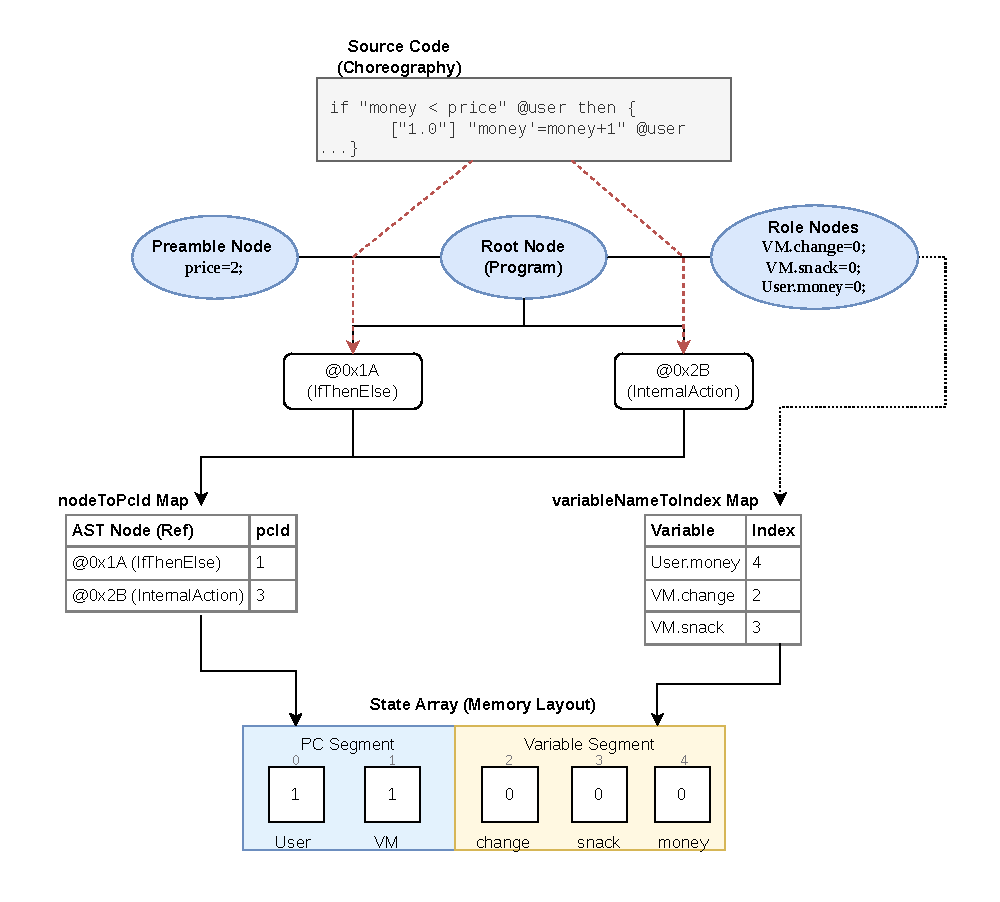
\includegraphics[width=0.9\textwidth]{figures/mapping5.drawio.pdf}
	\caption{Structure of the initial state vector $S_{0}$ for the Vending Machine protocol, illustrating the logical partitioning into the program counter segment and the canonical variable segment.}
	\label{fig:mapping}
\end{figure}


The PC segment is immediately followed by the variable segment, governed by the \texttt{variable\-Name\-To\-Index} map, which provides storage for all global and local variables. To ensure a canonical state representation, which is vital for efficient duplicate detection, we organize the variables lexicographically by their participating role and variable name. This strict ordering ensures that identical system states always result in identical vector representations, regardless of their discovery order.
By determining the \texttt{total\-Vector\-Size} as the sum of the PC indices and the variables upfront, we ensure that the vector's layout remains constant throughout the exploration. As illustrated in \cref{fig:mapping}, this flat structure allows for $O(1)$ access to any part of the system state, which is essential for the high-performance evaluation of guards and the application of assignments during the state space expansion.



\subsection{Stable Node Resolution and Guard Evaluation}
\label{subsec:control-flow}

To optimize the state space exploration, the engine distinguishes between \textit{stable} and \textit{unstable} AST nodes. This distinction is central to our state space reduction strategy. \textit{Unstable nodes} represent administrative or control-flow constructs---such as conditionals (\texttt{IfThenElseNode}) or protocol definitions (\texttt{RecNode})---that do not constitute a distinct, observable state of the distributed system. Instead of materializing these nodes as separate entries in the state space, the engine resolves them internally through a \textit{look-ahead} mechanism.
Execution only halts, and a new state vector is only materialized, upon reaching a \textit{stable node}. Stable nodes correspond to actual behavioral steps, such as communication statements or internal actions. By skipping purely structural transitions and only capturing stable configurations, the engine ensures that the resulting state space remains compact and focuses exclusively on the meaningful interactions and state changes of the choreography.
The core logic of this \emph{look-ahead} mechanism is shown in the simplified \cref{lst:resolve-stable-node}. 

\begin{listing}[h]
\begin{minted}{java}
	function resolveToNextStable(node, state):
		current = node
		while current is unstable:
			if current is Protocol or Recursion:
				current = resolveContinuation(current)
			else if current is If-Then-Else:
				if evaluate(current.guard, state):
					current = current.thenBranch
				else if current.hasElseBranch:
				current = current.elseBranch
				else:
					return null // Blocking Guard
		return current // Found stable action or branch
\end{minted}
\caption{Resolution of unstable AST nodes during state space exploration, including the handling of blocking guards via the \texttt{null} return value.}
\label{lst:resolve-stable-node}
\end{listing}

In the recursive Vending Machine protocol, exploration starts at the \texttt{Start} protocol. At this point, the engine first encounters the guard \texttt{money < price}, represented by an unstable \texttt{If\-Then\-Else\-Node}. Since such nodes only determine the control flow, they do not themselves give rise to a transition. Instead, the guard is evaluated against the current state vector. If the condition holds, the engine continues into the corresponding branch and skips over the unstable control-flow nodes until it reaches the next stable node.

In this example, the next stable node is an \texttt{InternalActionNode} that increments the \texttt{money} variable of the \texttt{user}. This action is only executed if the active process is indeed the \texttt{user}. If another process is currently considered active, the action is not performed. When the role matches, the variable update is applied and the program counter of the active process is advanced to the next control location.

\begin{figure}[h]
\centering
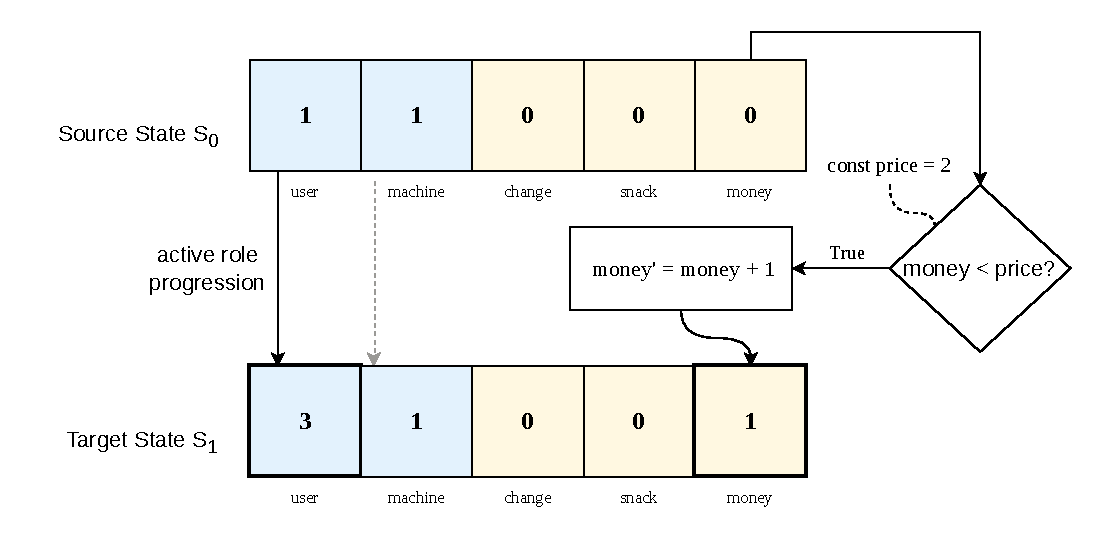
\includegraphics[width=0.9\textwidth]{figures/next_stable.drawio.pdf}
\caption{Atomic transformation of the state vector during a variable update step in the \texttt{Start} protocol. The engine evaluates the guard using the current variable segment and the global constant \texttt{price}. While the active role (\texttt{user}) advances to the next stable node ($\text{ID} 1	\rightarrow 3$) and updates the \texttt{money} variable, the passive role (\texttt{machine}) remains at its previous control location (ID $1$).}
\label{fig:start-protocol}
\end{figure}
As a result, the \texttt{user}'s program counter no longer points to the initial guard location, but to the next resolved position in the AST, namely node 3. The \texttt{machine}, by contrast, remains at node 1, since it has not yet taken part in the current step. In this way, the successor state reflects both the completed internal action of the active process and the unchanged waiting position of the other role.

Once a stable node has been reached, the engine constructs a successor state on a copy of the current state vector. It applies the required variable updates and advances the program counter of the active process to the next resolved location in the AST. The resulting vector is thus a fully formed successor state corresponding to one executable step of the model, rather than a purely intermediate control-flow configuration.

To construct the state transition graph, every discovered successor is passed to the \texttt{TransitionSink} alongside its associated transition rate. This component serves as the 'gatekeeper' of the state space: it performs duplicate detection by checking whether the state vector has already been visited. If the state is new, it is assigned a unique identifier and added to the worklist for further exploration. If the state has been encountered before, the engine simply reuses the existing identifier. By linking the source state to the (new or existing) target state, the \texttt{TransitionSink} incrementally builds the complete system model while ensuring that the exploration remains finite and efficient.

In the presence of recursion, this means that cycles arise when exploration returns to a state vector that is already known. Rather than introducing additional intermediate states for structural recursion steps, the implementation records a transition to the existing state, which makes the cyclic structure directly visible in the state space.

A crucial detail in the \texttt{resolveToNextStableNode} routine is the handling of unbalanced conditionals. If a guard evaluates to \texttt{false} and no \texttt{else} branch is defined, the method returns \texttt{null} (see \cref{lst:resolve-stable-node}). In the context of the state-space exploration, this \texttt{null} value indicates a \emph{blocking guard}: the active process cannot proceed along this execution path in the current state. Consequently, the interleaving engine does not generate any transitions for this process from the given source vector, effectively pruning invalid execution paths and ensuring that the model strictly adheres to the specified synchronization constraints.


\subsection{Synchronized Interaction and Probabilistic Branching}

We realize interactions between roles as synchronized updates of the state vector. When the exploration engine encounters a \texttt{BranchNode}, we identify the designated sender and receiver and check whether both processes are ready to participate in the same interaction. We generate a transition only if the receiver is at a compatible control-flow position. More precisely, the receiver's current program counter must either already point to the same \texttt{BranchNode} or be able to reach it by resolving only unstable nodes, such as \texttt{RecNode}, \texttt{ProtocolNode}, or \texttt{IfThenElseNode}, without executing any intervening stable action.

This alignment of control flows ensures that communication steps preserve the intended handshake semantics of the choreography. In contrast to internal actions, which affect only the active process, a synchronized interaction updates the control locations of both participating roles and may additionally apply the variable assignments associated with the selected branch.

\begin{figure}[ht!]
	\centering
	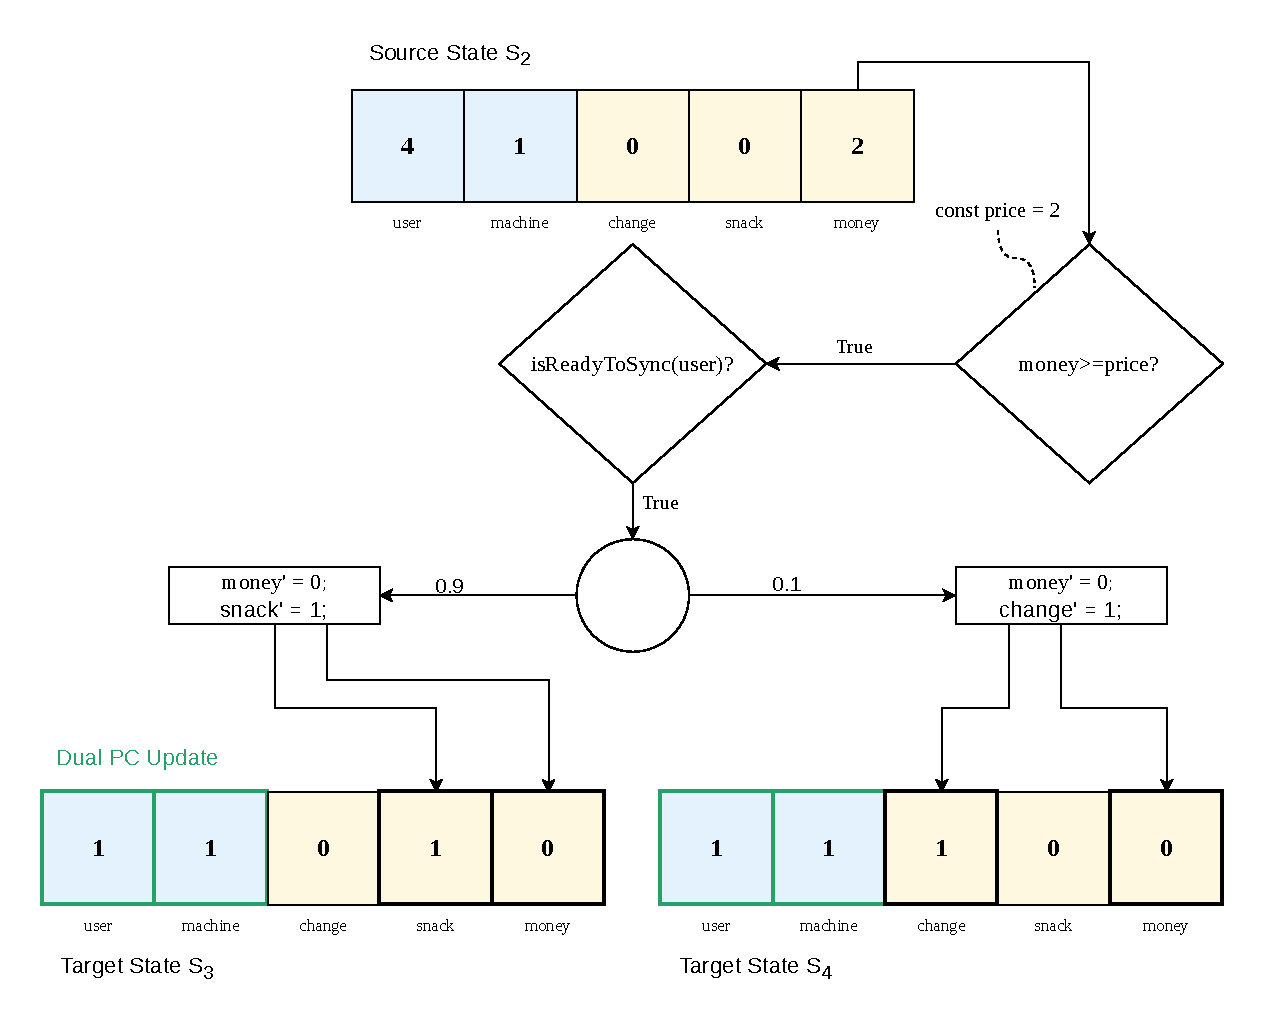
\includegraphics[width=0.95\textwidth]{figures/branching.drawio.pdf}
	\caption{Exploration of a synchronized interaction. Starting from state $S_{2}$	, the engine validates the global guard (\texttt{money >= price}) and the receiver's readiness (\texttt{isReadyToSync}). Upon a successful handshake, the exploration branches into two probabilistic outcomes ($S_{3}|S_{4}$) based on the specified rates (0.9 and 0.1). Each branch triggers a \textit{Dual PC Update} (highlighted in green), where the control locations of both participating roles are updated simultaneously alongside the respective variable assignments.}
	\label{fig:atomic-step}
\end{figure}


In the recursive \texttt{VendingMachine} protocol, this behavior becomes relevant in the \texttt{Payout} phase. We can only realize the communication between \texttt{machine} and \texttt{user} once the accumulated value of \texttt{money} satisfies the guard required to leave the \texttt{Start} phase. Only then can the \texttt{user}'s control flow advance to a position compatible with the \texttt{machine}'s branch, thereby enabling the synchronized interaction.

If this compatibility condition is satisfied, we generate one successor for each probabilistic branch of the interaction (see \cref{fig:atomic-step}). Each successor reflects the selected communication outcome by applying the corresponding assignments and updating the program counters of both roles to their respective continuations. In this way, we represent synchronized communication as a single atomic exploration step in the generated state space.


\subsection{Recursive Control Flow and State-Space Convergence}

We realize recursion by redirecting the program counter (PC) to the entry point of the referenced protocol rather than by introducing stack-based calls. Whenever the exploration reaches a \texttt{RecNode}, the engine resolves the identifier to its corresponding entry point. The program counter of the active process is then reset to the beginning of the respective protocol, ensuring a clean re-entry into the specified control flow.

This mechanism is directly observable in the payout interaction discussed in the previous section. As shown in \cref{fig:atomic-step}, the target states $S_3$ and $S_4$ both feature a program counter of ID 1 for both the \texttt{user} and the \texttt{machine}. This update is the technical result of the recursive call (\texttt{. Start}) at the end of the \texttt{Payout} phase. Instead of pushing a return address to a stack, the engine's routine to resolve continuations (\texttt{resolve\-Continuation}) identifies ID 1 as the stable entry point of the \texttt{Start} protocol and performs a direct PC-substitution. This approach is sufficient because recursion in our choreographic language does not function as a classical subroutine call that requires returning to a caller's context. Instead, recursive calls represent a transition to a renewed protocol behavior. Since there is no subsequent logic to be executed after a recursion is triggered, there is no need to maintain a call stack or track return addresses.

To ensure convergence for cyclic protocols, we maintain a centralized set of previously discovered state vectors. Before a newly generated successor is explored further, we check whether its vector representation has already been encountered. If it is new, it is inserted into the visited-state set and added to the worklist. Otherwise, the existing state is reused and the corresponding transition closes a cycle in the transition matrix.

This mechanism is essential because recursion may return the control flow to an earlier protocol position without reproducing the same global system state immediately. Even if the program counters assume values that have appeared before, exploration must continue as long as the variable segment differs. For instance, a state in which \texttt{snack = 1} is distinct from an otherwise structurally similar state in which \texttt{snack = 0}. Convergence is therefore reached only when the complete state vector, including both control locations and variable valuations, matches a previously discovered configuration. 

The resulting Discrete-Time Markov Chain (DTMC), shown in \cref{fig:vending-full-markov}, represents the complete state space of the Vending Machine protocol. To improve readability, the states are color-coded according to their logical role within the protocol. The grey nodes (0--2) denote the initial synchronization and setup phase that is shared by all execution paths. The blue and yellow clusters distinguish different behavioral branches of the choreography, in particular the \textit{Payout} and \textit{Refund} routines. Probabilistic branching points are highlighted by green edges, which correspond to the stochastic choices specified in the ARIA model, such as the 0.9/0.1 distribution used to represent the payout probabilities. Blue edges indicate recursive transitions. These cycles show that the exploration engine is able to close the state space by returning to previously discovered configurations via direct program-counter substitution, thereby yielding a finite exploration despite the recursive structure of the protocol.
The corresponding \texttt{.sta} and \texttt{.tra} files are provided in the \cref{sec:tra-sta-vending-machine}.

\begin{figure}[ht!]
	\centering
	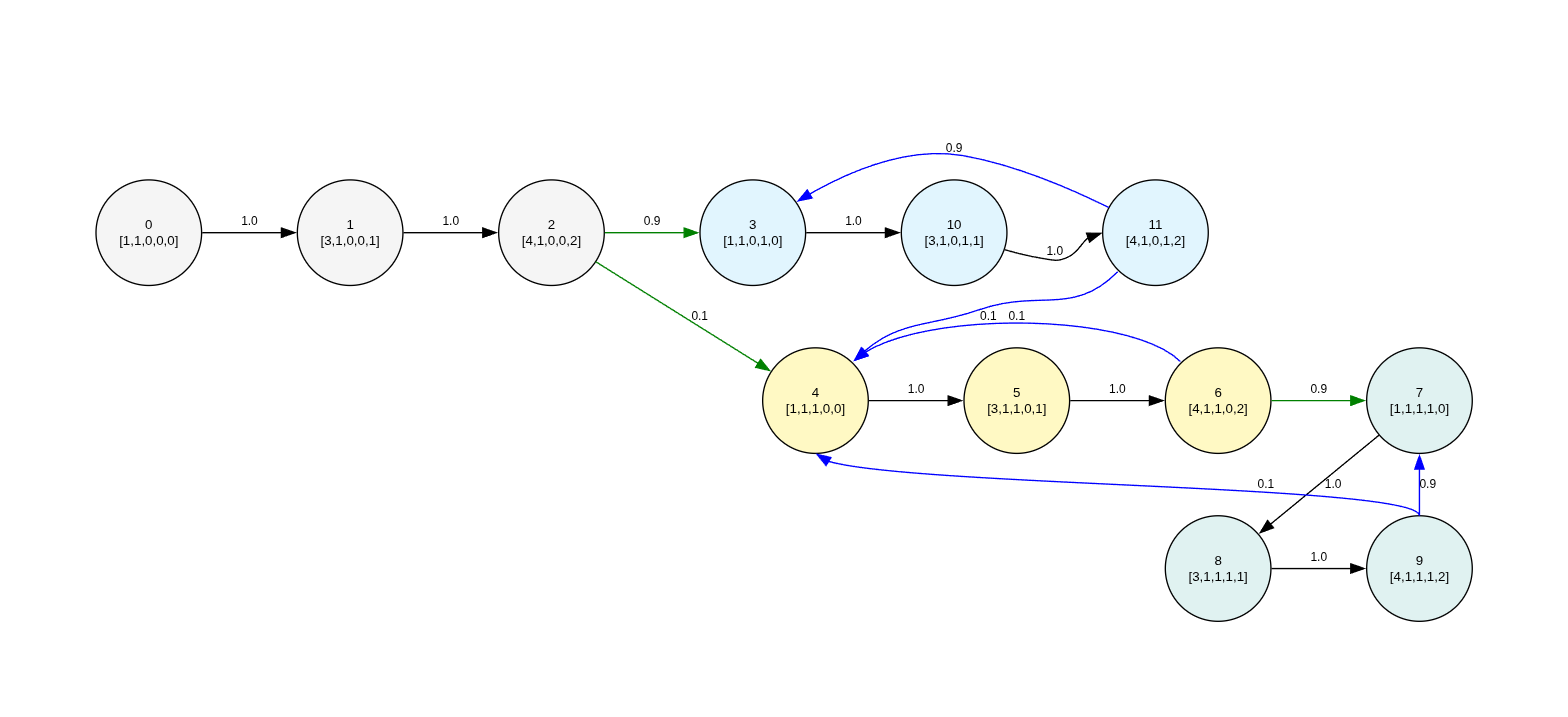
\includegraphics[width=0.95\textwidth]{figures/markovChain.png}
	\caption{Induced Markov chain of the recursive Vending Machine protocol}
	\label{fig:vending-full-markov}
\end{figure}


\section{Challenges}
\label{sec:challenges}
While the formal semantics define which states and transitions must be generated, an efficient implementation also depends on how these structures are stored, traversed, and serialized. This section therefore discusses two practical challenges that emerged during the implementation of \textsc{ARIA}: the decoupling of transition generation from file output, and the memory-efficient handling of explicit states during exploration.
\subsection{Producer--Consumer Decoupling for Transition Output}

A practical challenge in explicit-state exploration is the mismatch between CPU-bound successor generation and I/O-bound transition serialization. If every discovered transition were written to disk immediately, the exploration engine would repeatedly block on file output, reducing overall throughput.

To avoid this, we decouple exploration and serialization using a producer--consumer architecture. The exploration engine acts as the producer, while a dedicated background thread consumes transition records and writes them to the output file. Communication between both components is realized via a bounded \texttt{LinkedBlockingQueue}.

This design serves two purposes. First, it allows exploration to continue while previously generated transitions are being serialized. Second, the bounded queue limits the amount of buffered output and therefore prevents unbounded memory growth if file output temporarily becomes slower than state-space generation.

To terminate the consumer thread in a controlled manner, we use a sentinel record following the \texttt{POISON\-PILL}~\cite{goetz2006java} pattern. Once exploration is complete and no further transitions remain to be emitted, this special record is inserted into the queue, signaling the consumer to finish processing and close the output stream.


\subsection{Memory Efficiency and State Deduplication}
\label{sec:efficiency}

Since explicit-state exploration is inherently vulnerable to state-space explosion, memory efficiency is a central concern of the implementation. In our setting, each state is represented as an \texttt{Object[]} vector containing both control-flow information and variable valuations.

Initially, we attempted to use standard Java collection types, such as \texttt{HashSet<>}, for state storage. However, this approach was insufficient because Java arrays rely on identity-based hashing and equality by default. Consequently, logically identical states reconstructed at different points during the exploration were treated as distinct instances, causing the deduplication to fail and leading to redundant exploration and rapid memory exhaustion. To resolve this, we implemented a custom hashing strategy that compares vectors by their actual contents rather than by object identity. This ensures that two independently constructed vectors are recognized as the same logical state whenever both their program-counter segment and their variable segment coincide.

Beyond state storage itself, the order of exploration also affects memory consumption. Our starting point was a standard breadth-first search (BFS) strategy. While BFS is ideal for finding shortest paths to a state, it requires the engine to store the entire frontier of the search tree in the worklist. For concurrent choreographies with high branching factors, this "frontier explosion" consumed several gigabytes of RAM before any significant depth was reached.

To keep the worklist size manageable, we moved to a biased hybrid search strategy. The worklist is implemented as an \texttt{ArrayDeque}, which allows us to alternate between depth-first and breadth-first expansion. In practice, we predominantly explore states in a depth-first manner (DFS), while periodically taking breadth-first steps to maintain coverage across different execution paths. This combination provides a pragmatic balance between exploration depth and memory stability. A purely breadth-first traversal may cause the worklist to grow rapidly, whereas a purely depth-first traversal may delay the discovery of relevant alternative behaviors. By combining both strategies, we obtain a more robust exploration order while keeping the active frontier within manageable bounds.
